
\documentclass[10pt]{beamer}

\mode<presentation>
{
 \usetheme{Boadilla}
\pagestyle{empty}

\setbeamerfont*{frametitle}{size=\normalsize,series=\bfseries}
\setbeamerfont*{block}{size=\normalsize,series=\bfseries}
%\setbeamertemplate{blocks}[rounded][shadow=true]
}

\definecolor{links}{HTML}{2A1B81}
\hypersetup{colorlinks,linkcolor=,urlcolor=links}


\usepackage{etex}
% \usepackage{helvet}
\usepackage{amsmath, amssymb}
\usepackage{color}
\usepackage{asymptote}
\usepackage{mathrsfs}
\usepackage{dsfont}
\usepackage{makeidx}
\usepackage{multido}
\usepackage{dsfont}


\usepackage{pst-sigsys,pst-plot,pstricks-add}
%\usepackage{auto-pst-pdf}
\usepackage{pst-pdf}



\definecolor{links}{HTML}{2A1B81}
\hypersetup{colorlinks,linkcolor=,urlcolor=links}

\def\nn{\nonumber}

\definecolor{links}{HTML}{2A1B81}
\hypersetup{colorlinks,linkcolor=,urlcolor=links}

\newcommand{\fs}[2]{#2}


\title[]{LTI systems and the convolution operation}
\author[\textcolor{blue}{Systems and Circuits}]{\textcolor{darkblue}{Pablo M. Olmos} (olmos@tsc.uc3m.es)\\ \textcolor{darkblue}{Emilio Parrado} (emipar@tsc.uc3m.es)}
\institute{\textcolor{white}{UC3M}}

\definecolor{darkblue}{rgb}{0.0, 0.0, 0.40}
\setbeamercolor{title}{fg=darkblue}
\setbeamercolor{frametitle}{fg=darkblue}
\definecolor{darkgreen}{rgb}{0.0, 0.4, 0.0}


\AtBeginSection[]
{
  \begin{frame}<beamer>{Index}
    \tableofcontents[currentsection,currentsubsection]
  \end{frame}
}

\begin{document}
\frame{
\titlepage
\thispagestyle{empty}
\begin{center}

\includegraphics[scale=0.05]{Figures/uc3m-logo.pdf}
\end{center}
}

\section{Introduction to LTI systems}


\frame{
\frametitle{Motivation: Image Filtering}

\begin{figure}
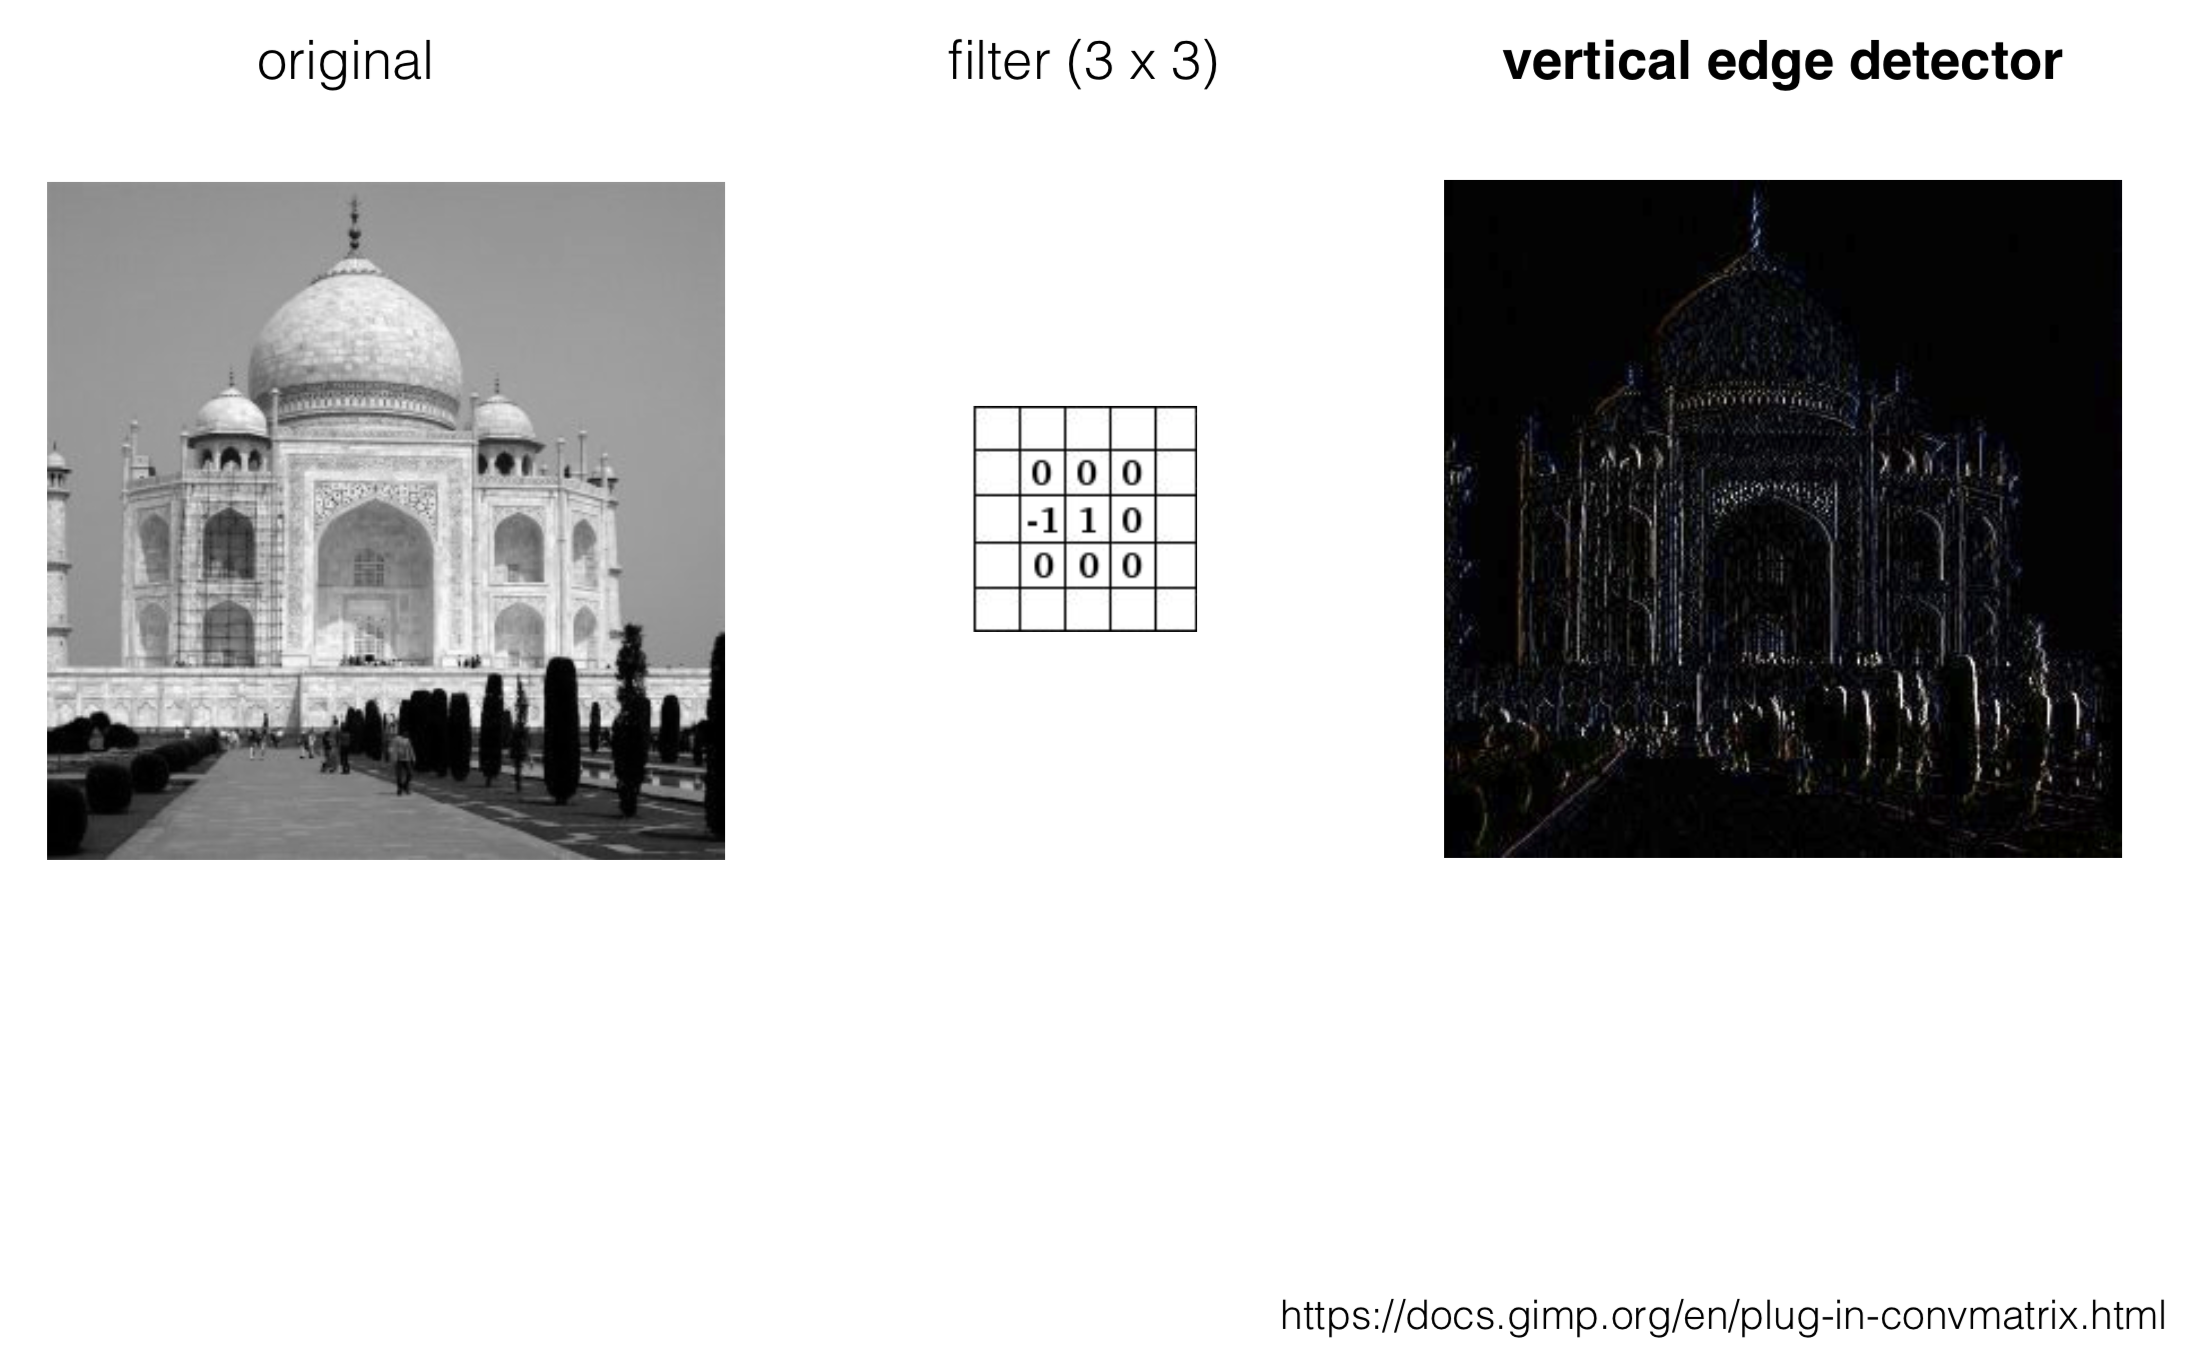
\includegraphics[scale=0.3]{Filtro_1.png}
\end{figure}

}

\frame{
\frametitle{Motivation: Image Filtering}

\begin{figure}
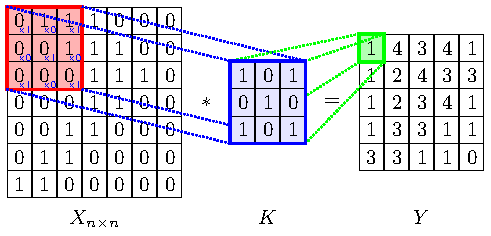
\includegraphics[scale=1.0]{2D_1.pdf}
\end{figure}

\begin{align*}
Y[1,1]&=X[1,1]*K[1,1]+X[1,2]*K[1,2]+X[1,3]*K[1,3]\\
&+X[2,1]*K[2,1]+X[2,2]*K[2,2]+X[2,3]*K[2,3]\\
&+X[3,1]*K[3,1]+X[3,2]*K[3,2]+X[3,3]*K[3,3]
\end{align*}
}

\frame{
\frametitle{Motivation: Image Filtering}

\begin{figure}
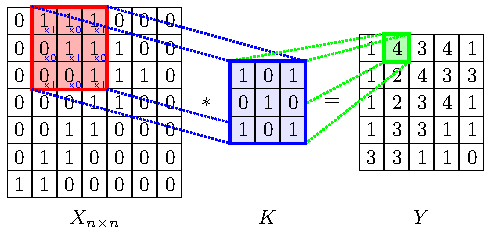
\includegraphics[scale=1.0]{2D_2.pdf}
\end{figure}

\begin{align*}
Y[1,2]&=X[1,2]*K[1,1]+X[1,3]*K[1,2]+X[1,4]*K[1,3]\\
&+X[2,2]*K[2,1]+X[2,3]*K[2,2]+X[2,4]*K[2,3]\\
&+X[3,2]*K[3,1]+X[3,3]*K[3,2]+X[3,4]*K[3,3]
\end{align*}
}




\frame{
\frametitle{Motivation: Image Filtering}

\begin{figure}
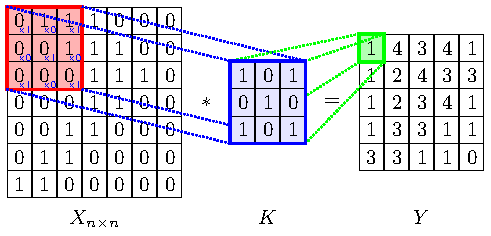
\includegraphics[scale=1.0]{2D_1.pdf}
\end{figure}

\begin{align*}
Y[i,j]&=\sum_{k_1=1}^{n}\sum_{k_2=1}^{n} X[k_1,k_2]K[i-k_1,j-k_2], ~~~ K[u,q]=0 \text{ para } u>3, q>3
\end{align*}

{\bf Linear operator, the result does not depend on the position of the image}
}

\frame{
\frametitle{Motivation: Image Filtering}

\begin{figure}
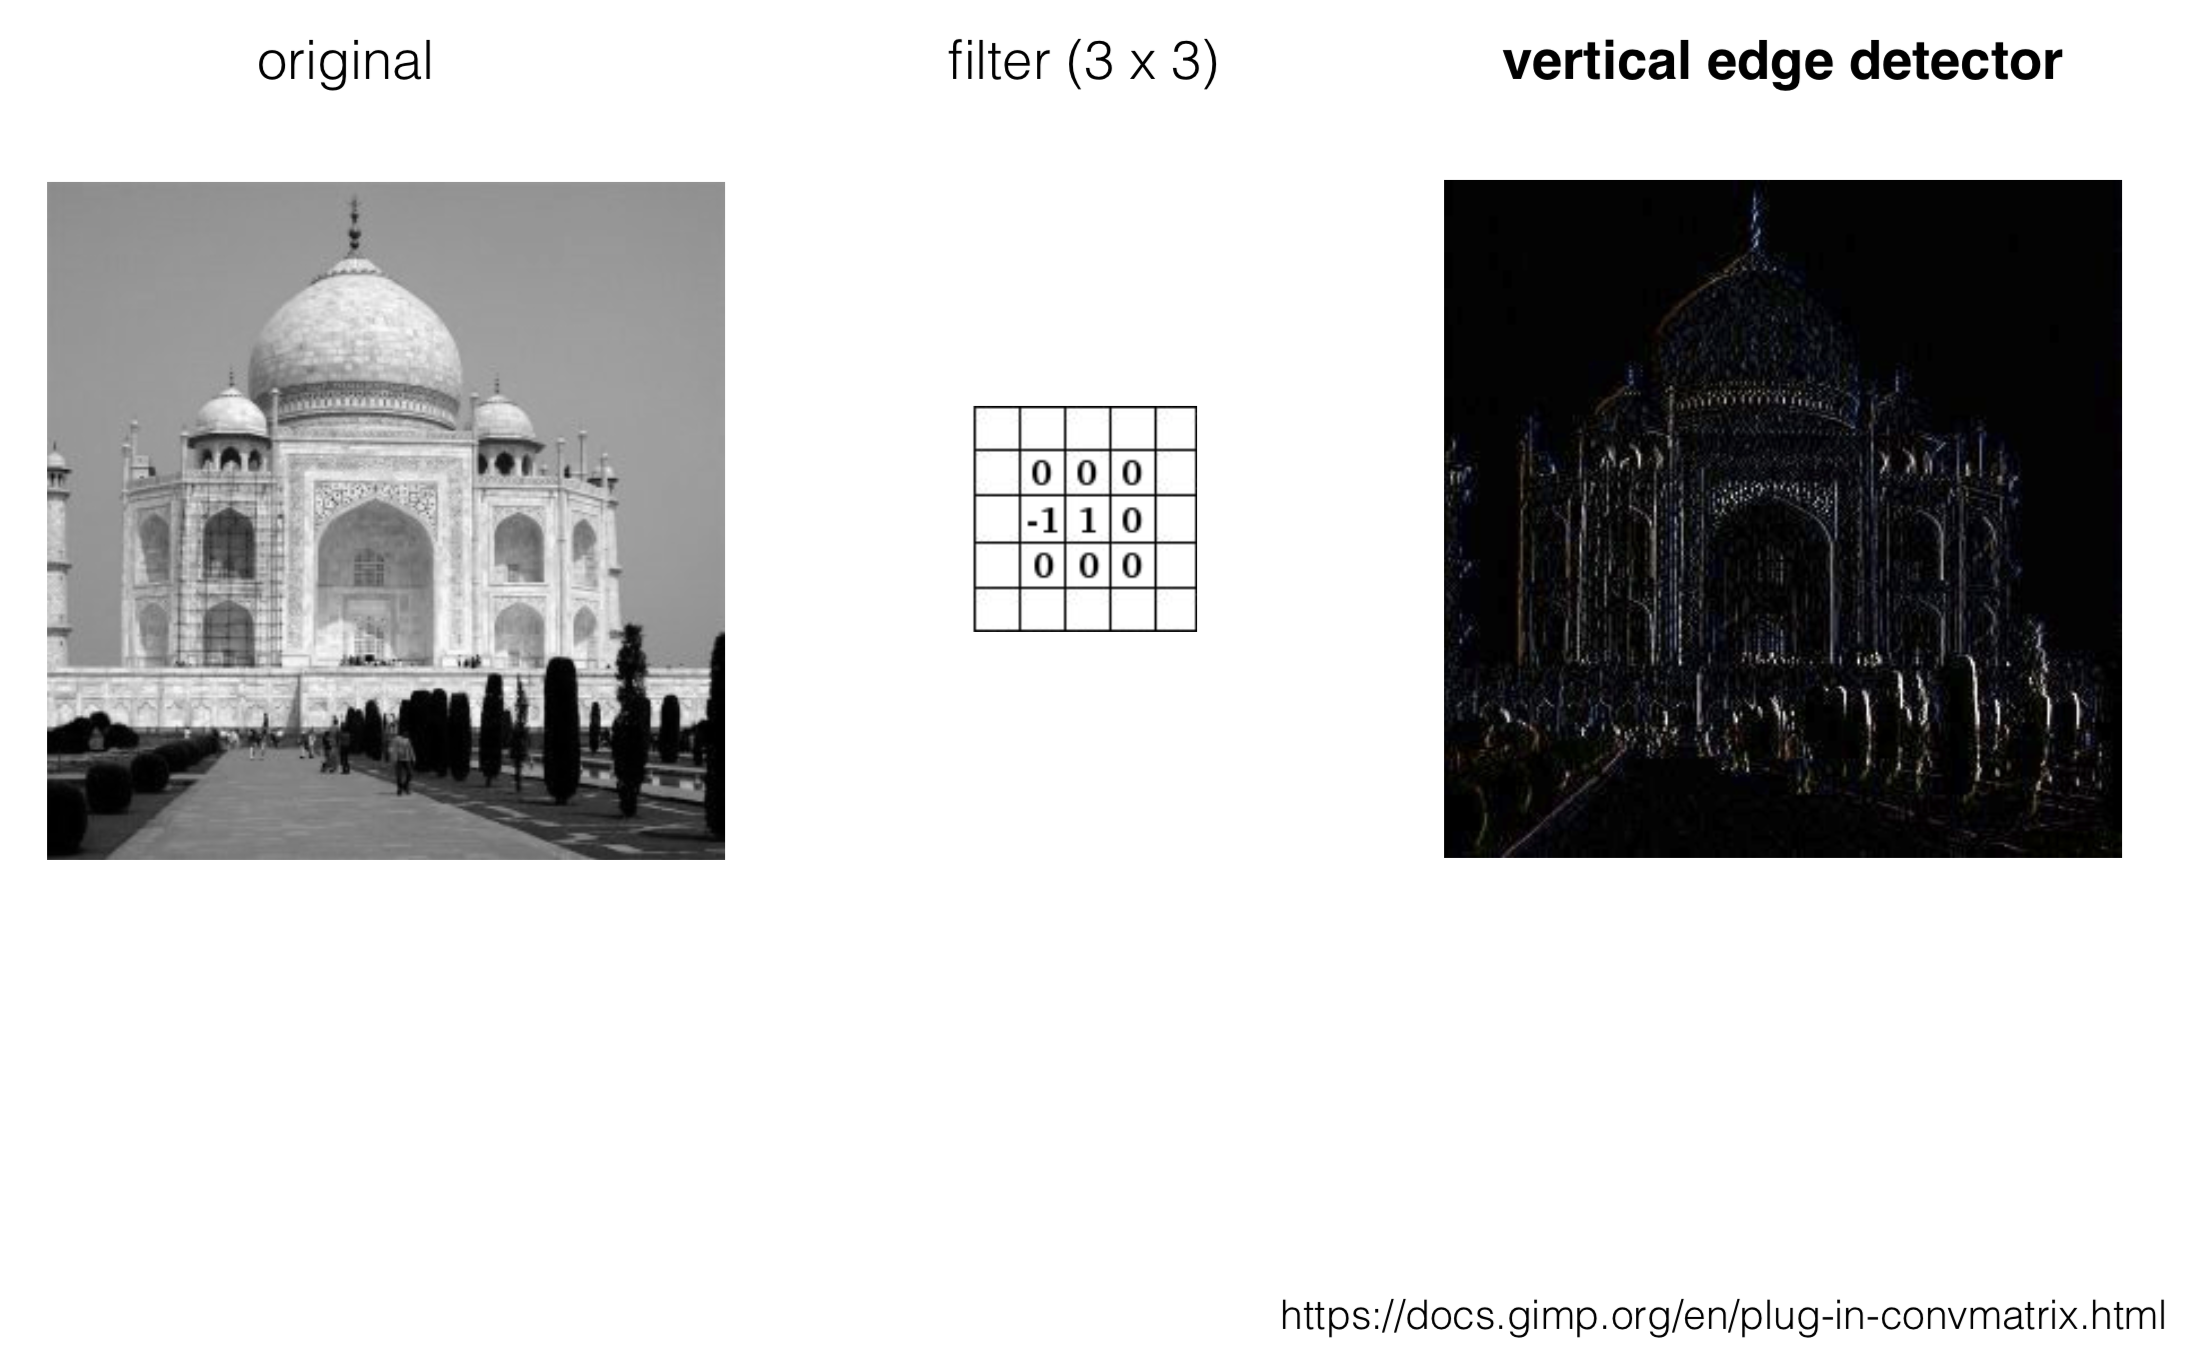
\includegraphics[scale=0.3]{Filtro_1.png}
\end{figure}

}

\frame{
\frametitle{Motivation: Image Filtering}

\begin{figure}
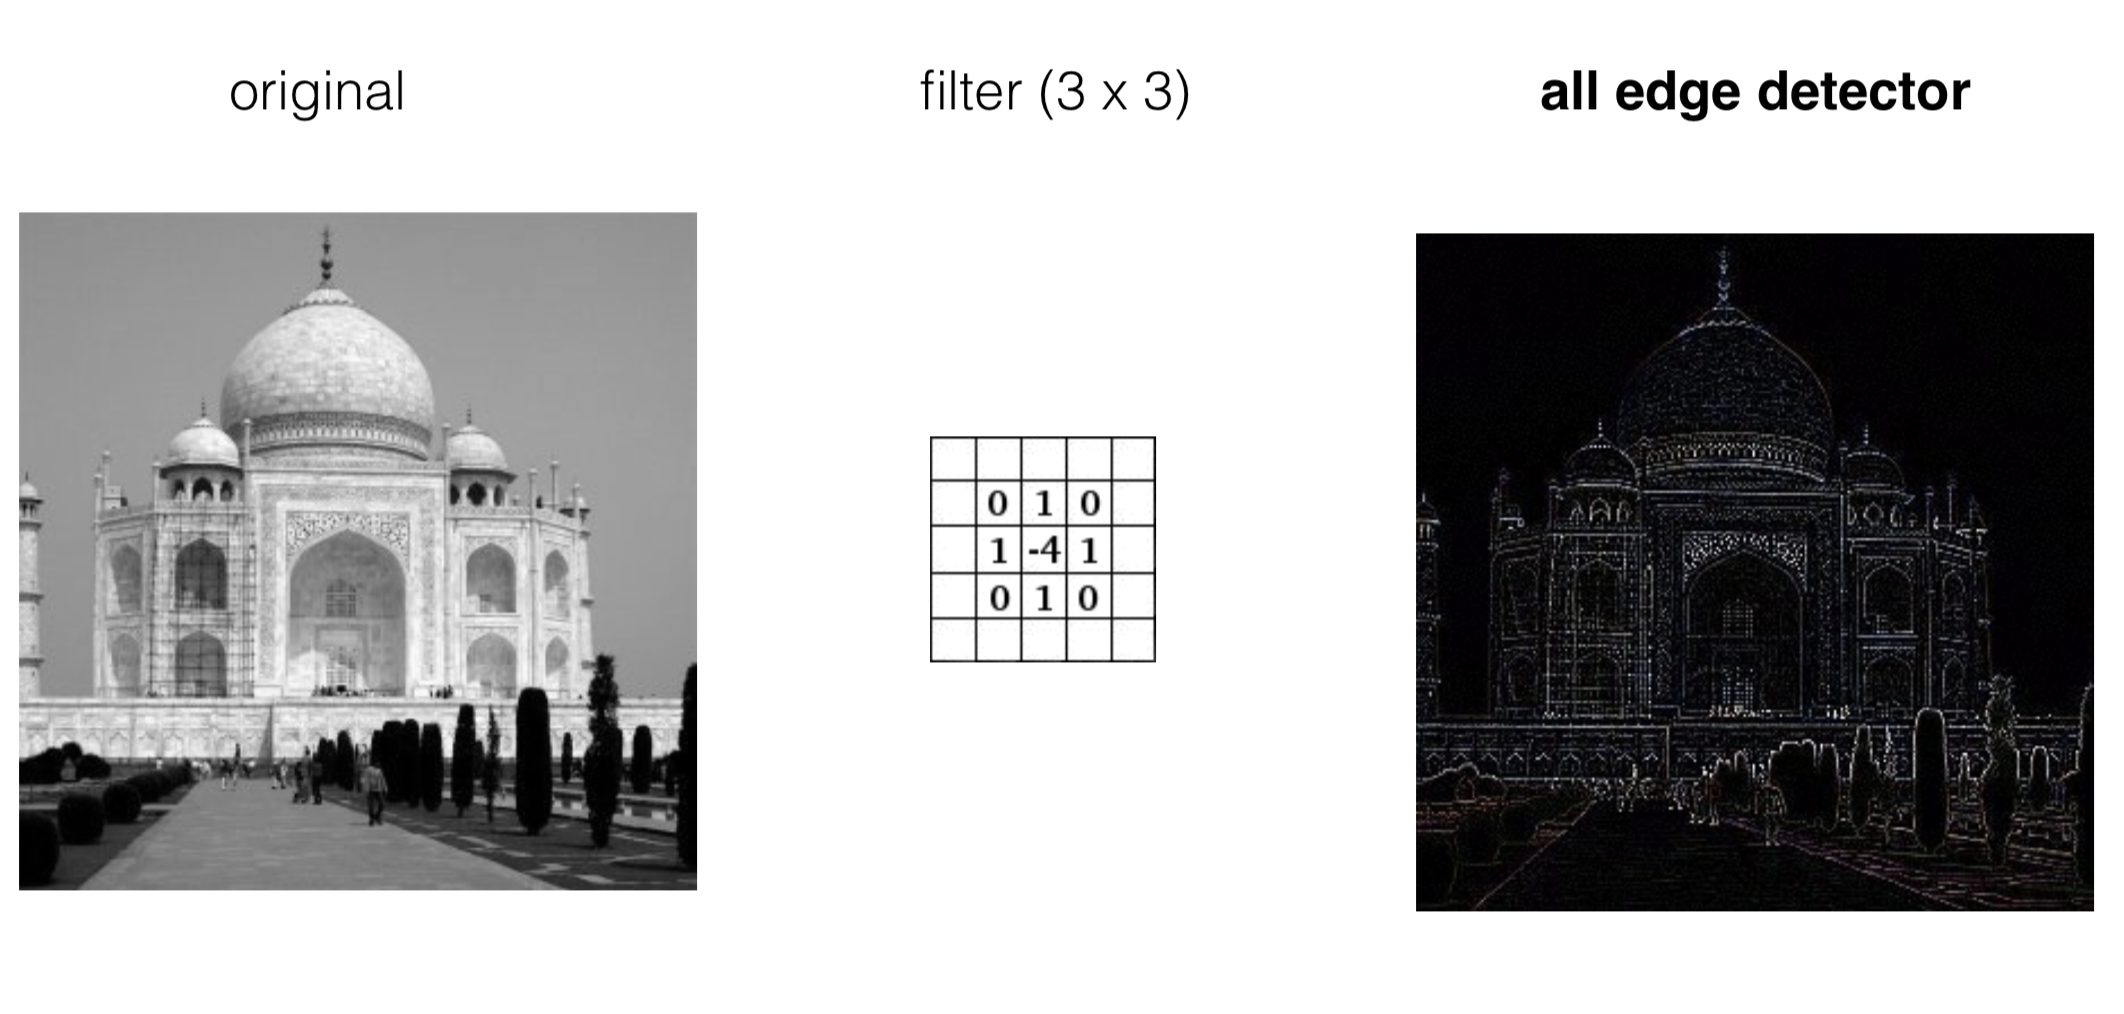
\includegraphics[scale=0.3]{Filtro_2.png}
\end{figure}

}

\frame{
\frametitle{Motivation: Image Filtering}

\begin{figure}
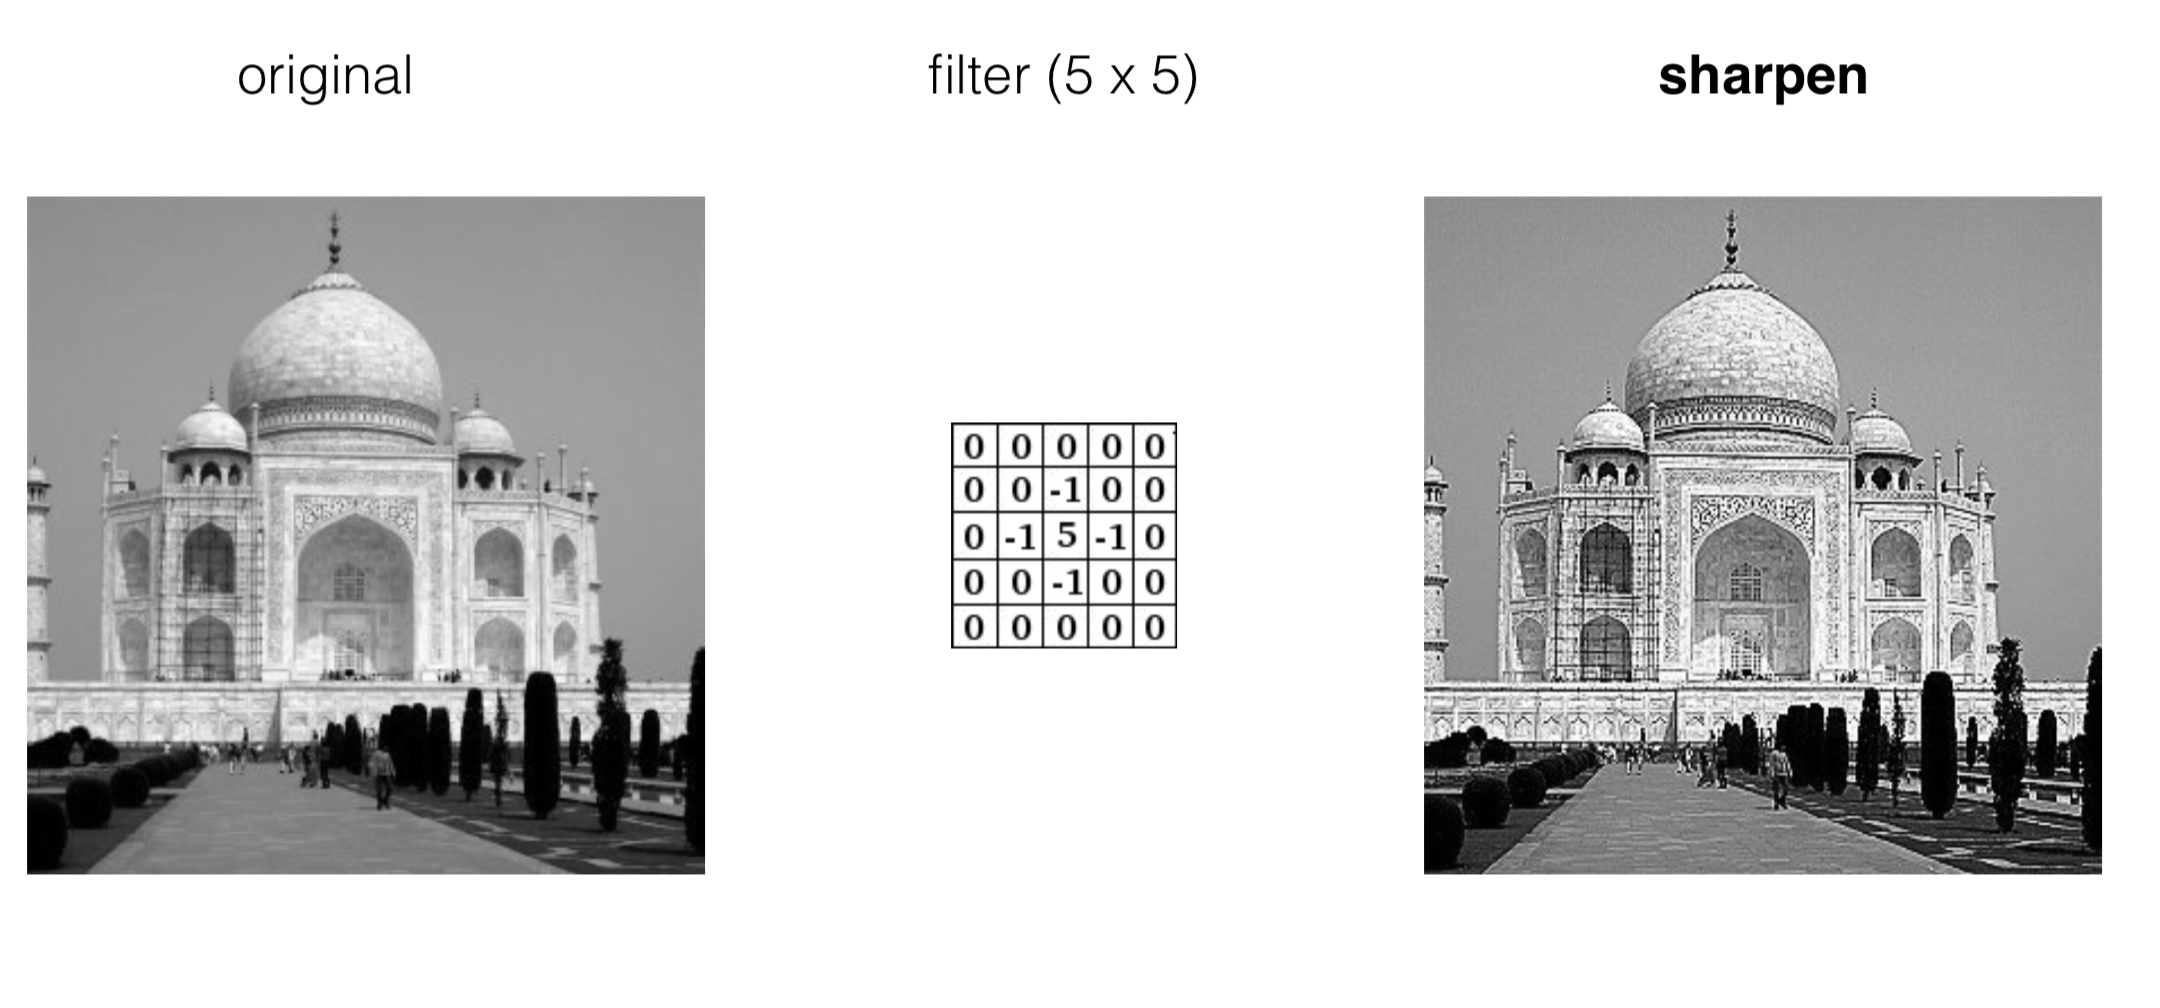
\includegraphics[scale=0.3]{Filtro_3.png}
\end{figure}

}


\frame{
\begin{itemize}
\item The theory of LTI systems has direct applications in a wide set of technical areas: 
\begin{itemize}
\item Nuclear magnetic resonance spectroscopy
\item Seismology
\item Electric circuit design
\item Control Theory
\item Any application that involves Signal Processing
\end{itemize}
\item Our goal in Systems and Circuits: predict the output of a given LTI system for a given input.
\item In future courses you will face the design of LTI systems according to certain specifications.
\end{itemize}
}

\frame{
\frametitle{Time Invariance}

\begin{block}{}
A system is time-invariant if a time shift in the input signal causes a time shift in the output signal.
\end{block}
\vspace{0.5cm}

\begin{itemize}
\item Given $y[n]=f(x[n])$, the system is time-invariant if $f(x[n-n_0])=y[n-n_0]$ $\forall~n_0$. 
\item Given $y(t)=f(x(t))$, the system is time-invariant if $f(x(t-t_0))=y(t-t_0)$ $\forall~t_0$. 
\end{itemize}
}


\frame{
\frametitle{Linearity}
Linear system posses the important property of superposition.

\begin{exampleblock}{}
 For any system, consider two arbitrary inputs and their respective outputs:
\begin{align}\nn
x_1(t)\rightarrow y_1(t)\\\nn
x_2(t)\rightarrow y_2(t),
\end{align}
the system is linear if 
\begin{align}\nn
ax_1(t)+bx_2(t)\rightarrow ay_1(t)+by_2(t)
\end{align}
for any two complex constant $a,b\in\mathbb{C}$.
\end{exampleblock}

\begin{block}{Linear discrete-time signals}
\begin{align}\nn
ax_1[n]+bx_2[n]\rightarrow ay_1[n]+by_2[n]
\end{align}
\end{block}

}



\frame{
\frametitle{Analysis of LTI systems}

\begin{figure}
\centering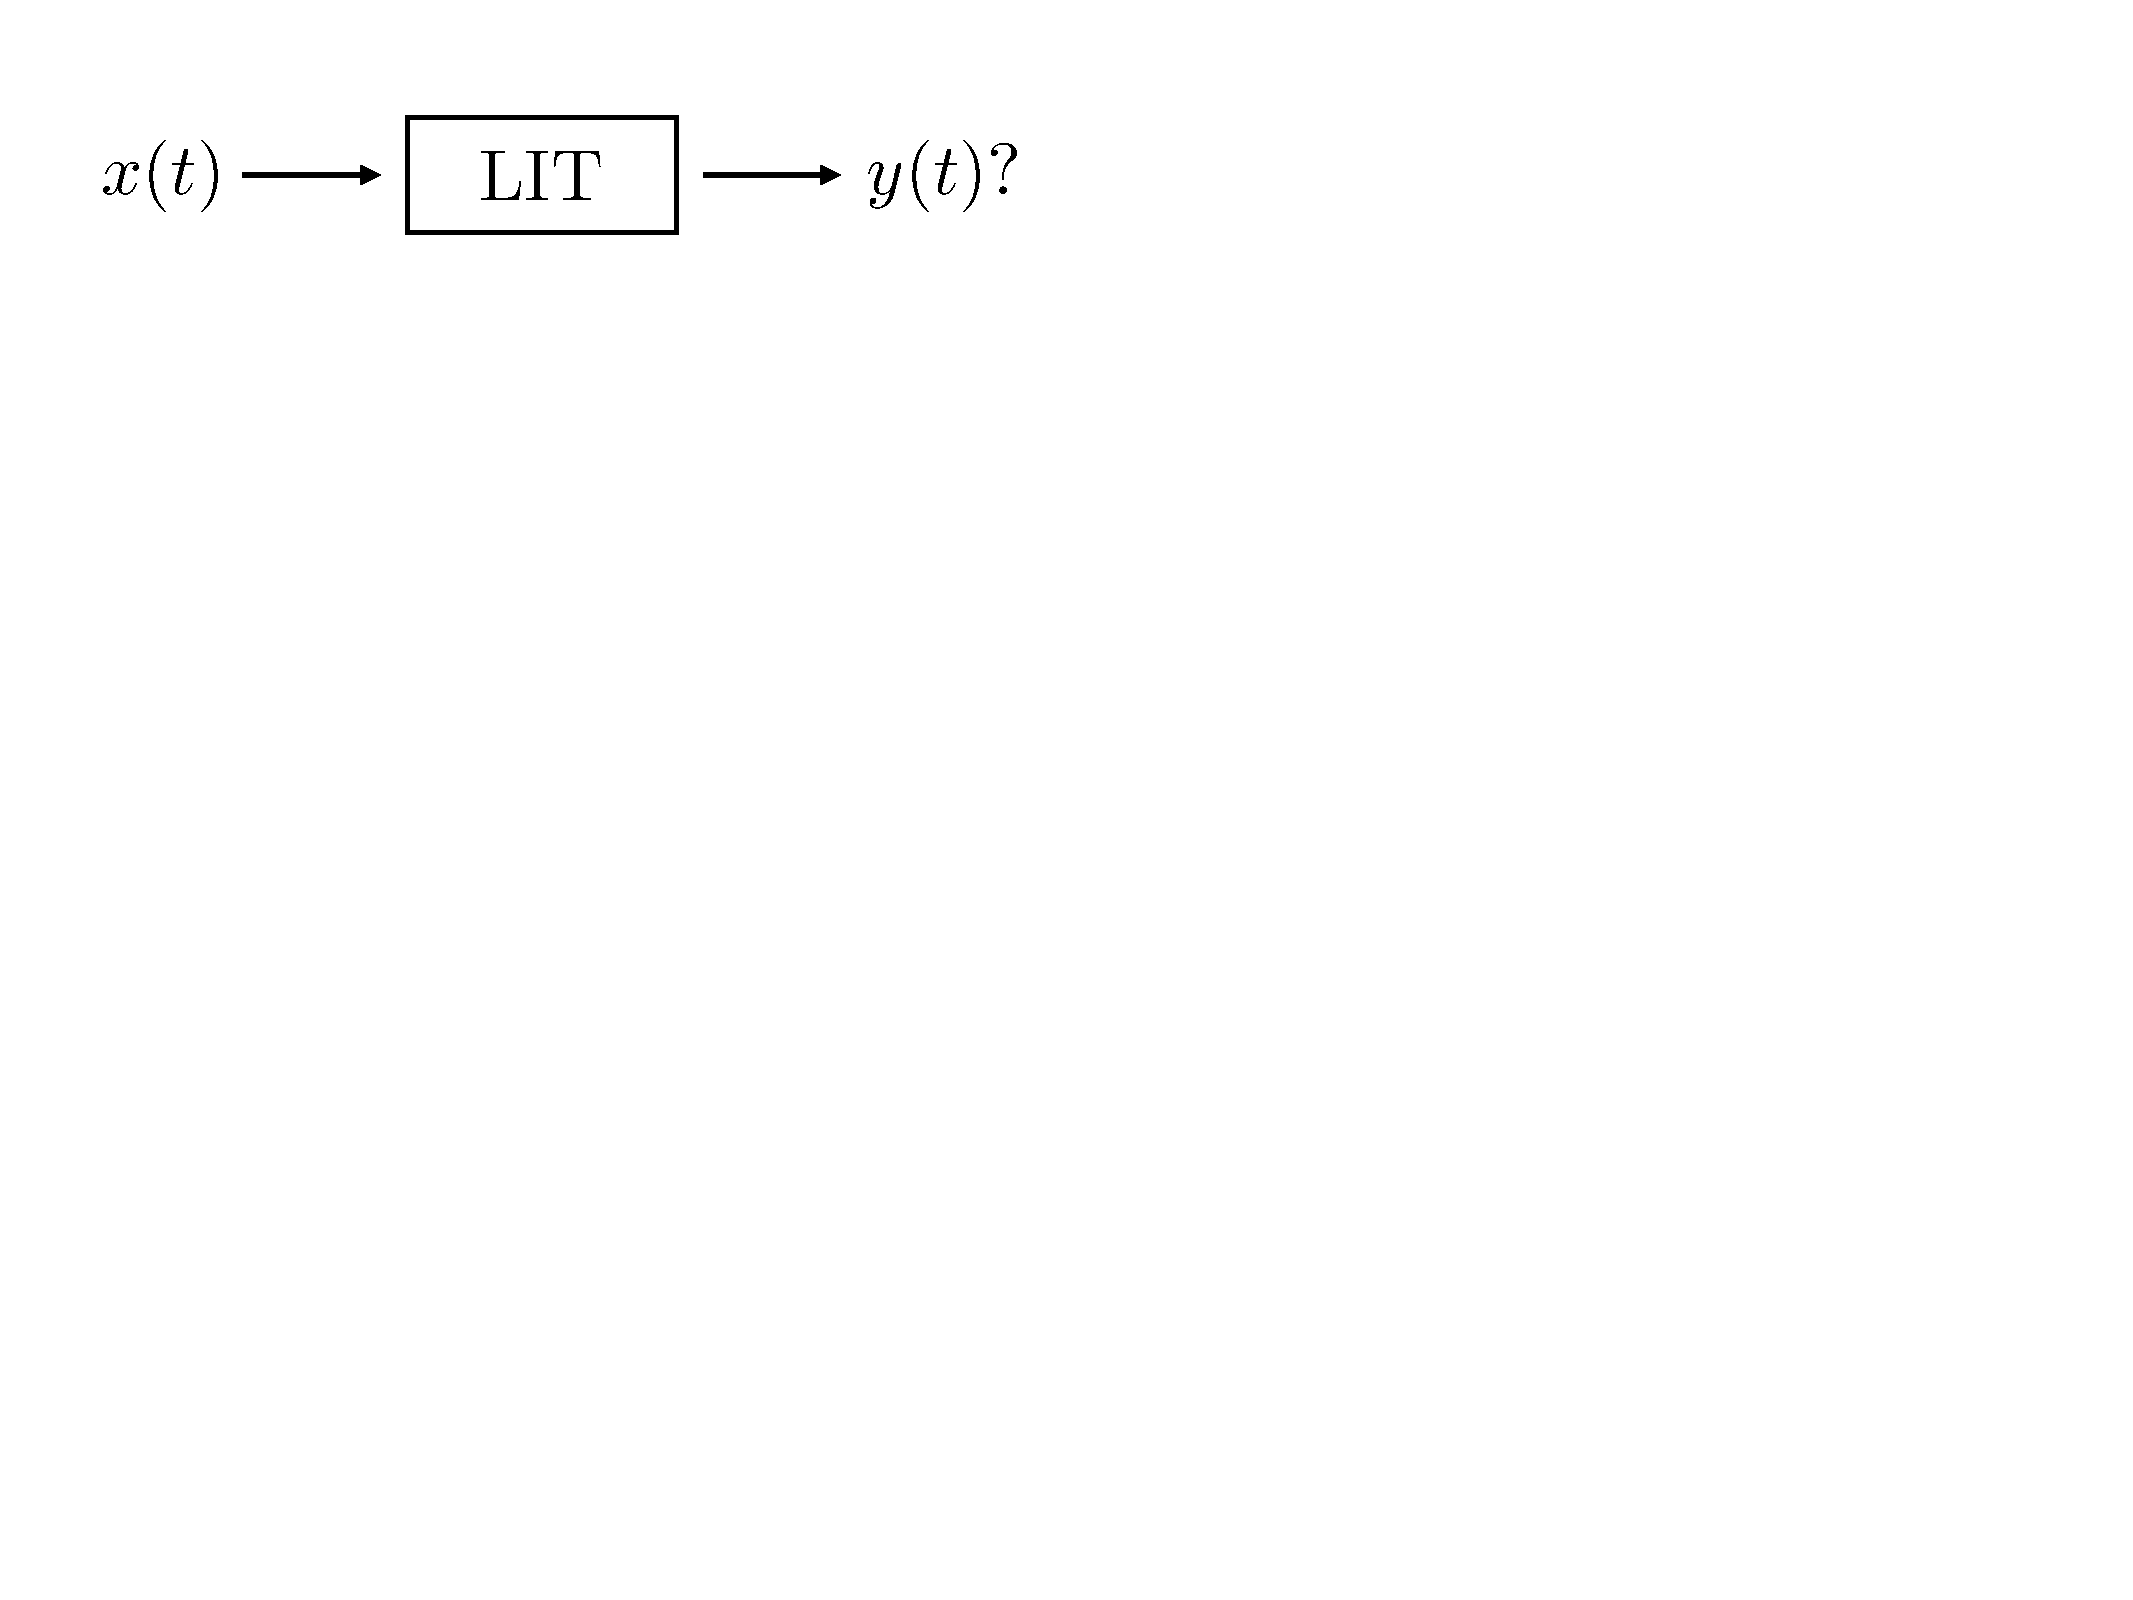
\includegraphics[scale=0.3]{P6.pdf}
\end{figure}

\vspace{0.5cm}
\begin{itemize}
\item Decompose input signal by means of a linear combination of simpler signals
\end{itemize}

$$x(t) = \dots a_{-1} \phi_{-1} (t) + a_{-2} \phi_{0} (t) + a_{0} \phi_{0} (t) + a_{1} \phi_{1} (t) + a_{2} \phi_{2} (t) + \ldots $$

\begin{itemize}
\item These ``basic" signals are chosen to provide a certain degree of analytical convenience, so we can  analyze the system's properties and its response to arbitrary input signals:
\begin{itemize}
\item Delayed Impulses $\Rightarrow$ \textbf{\textcolor{darkblue}{Convolution}}
\item Complex exponential signals $\Rightarrow$ \textbf{\textcolor{darkblue}{Fourier analysis}}
\end{itemize}
\end{itemize}


}

\section{Discrete-time LTI systems}

\frame{

\begin{pspicture}[](5,2)
   \pssignal(0,1){x}{$x[n]$}
   \psblock(2,1){a}{LTI}
   %\psblock(4,1){b}{$h[n], H(z)$}
   \pssignal(4,1){y}{$y[n]$?}
   %-----------------
   \psset{arrows=->}
   \ncline{x}{a}  \ncline{a}{y}  %\ncline{b}{y}
\end{pspicture}

\vspace{0.5cm}
Remember that any discrete-time sequence $x[n]$ can be decomposed as a linear combination of unit impulses:
\begin{block}{}
\begin{align}\nn
x[n]&=\sum_{k=-\infty}^{\infty}x[k]\delta[n-k]\\\nn
&=\ldots+x[-20]\delta[n+20]+x[-19]\delta[n+19]+\ldots\\\nn
&+x[-1]\delta[n+1]+x[0]\delta[n]+x[1]\delta[n-1]+\ldots
\end{align}
\end{block}
}

\frame{
\textbf{If the system is linear} and we are able to compute
\vspace{0.5cm}

\begin{center}
\begin{pspicture}[](6.5,5)
	
   \pssignal(0,5){x1}{$\delta[n]$}
    \psblock(2,5){a1}{LTI}
    \pssignal(4,5){y1}{$h_0[n]$}   
   \pssignal(0,4){x2}{$\delta[n+1]$}
    \psblock(2,4){a2}{LTI}
    \pssignal(4,4){y2}{$h_{-1}[n]$}      
     \pssignal(0,3){x3}{$\delta[n-1]$}
    \psblock(2,3){a3}{LTI}
    \pssignal(4,3){y3}{$h_{1}[n]$}     
    
    \ldotsnode[angle=90](0,2){dots}
    \ldotsnode[angle=90](2,2){dots}
    \ldotsnode[angle=90](4,2){dots}
    
    \pssignal(0,1){x4}{$\delta[n-k]$}
    \psblock(2,1){a4}{LTI}
    \pssignal(4,1){y4}{$h_{k}[n]$}   
    
   \psset{arrows=->}
   \ncline{x1}{a1}  \ncline{a1}{y1}    
   \ncline{x2}{a2}  \ncline{a2}{y2}  
    \ncline{x3}{a3}  \ncline{a3}{y3} 
     \ncline{x4}{a4}  \ncline{a4}{y4}  
       
\end{pspicture}
\end{center}

then we can make use of the superposition property!
}

\frame{


\begin{pspicture}[](9,2)
   \pssignal(0,1){x}{$x[n]=\displaystyle\sum_{k=-\infty}^{\infty}x[k]\delta[n-k]$}
   \psblock(4,1){a}{LTI}
   %\psblock(4,1){b}{$h[n], H(z)$}
   \pssignal(6,1){y}{$y[n]$}
   %-----------------
   \psset{arrows=->}
   \ncline{x}{a}  \ncline{a}{y}  %\ncline{b}{y}
\end{pspicture}

\vspace{0.5cm}
\begin{exampleblock}{}
\begin{align}\nn
y[n]=\sum_{k=-\infty}^{\infty}x[k]h_{k}[n]
\end{align}
\end{exampleblock}

\vspace{0.5cm}
\begin{itemize}
\item This is just a consequence of the system linearity.
\item The problem is reduced to evaluate the system's output for any $\delta[n-k]$.
\item The problem can be further reduced  by exploiting that the system is \textbf{time-invariant}.
\end{itemize}

}

\frame{

\begin{center}
\begin{pspicture}[](8,5)
	
   \pssignal(0,5){x1}{$\delta[n]$}
    \psblock(2,5){a1}{LTI}
    \pssignal(5,5){y1}{$h_0[n]=h[n]$}   
   \pssignal(0,4){x2}{$\delta[n+1]$}
    \psblock(2,4){a2}{LTI}
    \pssignal(5,4){y2}{$h_{-1}[n]=h[n+1]$}      
     \pssignal(0,3){x3}{$\delta[n-1]$}
    \psblock(2,3){a3}{LTI}
    \pssignal(5,3){y3}{$h_{1}[n]=h[n-1]$}     
    
    \ldotsnode[angle=90](0,2){dots}
    \ldotsnode[angle=90](2,2){dots}
    \ldotsnode[angle=90](4,2){dots}
    
    \pssignal(0,1){x4}{$\delta[n-k]$}
    \psblock(2,1){a4}{LTI}
    \pssignal(5,1){y4}{$h_{k}[n]=h[n-k]$}   
    
   \psset{arrows=->}
   \ncline{x1}{a1}  \ncline{a1}{y1}    
   \ncline{x2}{a2}  \ncline{a2}{y2}  
    \ncline{x3}{a3}  \ncline{a3}{y3} 
     \ncline{x4}{a4}  \ncline{a4}{y4}  
       
\end{pspicture}
\end{center}

Therefore, for any input $x[n]$, if $h[n]$ is known then the system output is given by

\begin{exampleblock}{}
\begin{align}\nn
y[n]=\sum_{k=-\infty}^{\infty}x[k]h_{k}[n]=\sum_{k=-\infty}^{\infty}x[k]h[n-k]
\end{align}
\end{exampleblock}

}

\frame{

\begin{itemize}
\item $h[n]$ is the system's \textbf{impulse response}.
\item Any LTI system is \textbf{completely defined} by $h[n]$!
\vspace{0.3cm}
\begin{center}
\begin{pspicture}[](5,2)
   \pssignal(0,1){x}{$x[n]$}
   \psblock(2,1){a}{$h[n]$}
   %\psblock(4,1){b}{$h[n], H(z)$}
   \pssignal(4,1){y}{$y[n]$}
   %-----------------
   \psset{arrows=->}
   \ncline{x}{a}  \ncline{a}{y}  %\ncline{b}{y}
\end{pspicture}
\end{center}
\end{itemize}


\begin{block}{Convolution}
Given two discrete-time signals $x[n]$ and $h[n]$:
\begin{align}\nn
\sum_{k=-\infty}^{\infty}x[k]h[n-k]=x[n]\ast h[n]
\end{align}
is the convolution operation between them.
\end{block}


}

%
%\frame{
%\frametitle{Example I}
%
%\psset{xunit=0.75cm,yunit=0.75cm}
%
%\begin{tabular}{|c|c|}
%\hline
%\begin{pspicture}[showgrid](-2,-1)(4,3)
%  \rput(0,0){\psaxeslabels(0,0)(-2,0)(4,0){$n$}{}
%     \rput[tl](-2,3){$x[n]$}
%     \psstem[style=Stem,linecolor=blue](-1,1)
%            {0,1,2,0}}
%\end{pspicture}
%&
%\begin{pspicture}[showgrid](-1,-1)(5,3)
%  \rput(0,0){\psaxeslabels(0,0)(-1,0)(5,0){$n$}{}
%     \rput[tl](-1,3){$h[n]$}
%     \psstem[style=Stem,linecolor=blue](0,1)
%            {0,1,1,1,0}}
%\end{pspicture}\\
%\hline
%\end{tabular}
%
%
%}
%
%\frame{
%%\frametitle{Example I}
%
%\begin{center}
%\begin{pspicture}[](5,2)
%   \pssignal(0,1){x}{$x[n]$}
%   \psblock(2,1){a}{$h[n]$}
%   %\psblock(4,1){b}{$h[n], H(z)$}
%   \pssignal(4,1){y}{$y[n]$}
%   %-----------------
%   \psset{arrows=->}
%   \ncline{x}{a}  \ncline{a}{y}  %\ncline{b}{y}
%\end{pspicture}
%\end{center}
%
%\psset{xunit=0.75cm,yunit=0.75cm}
%
%\begin{center}
%
%\begin{pspicture}[showgrid](0,-1)(6,3)
%  \rput(0,0){\psaxeslabels(0,0)(0,0)(6,0){$n$}{}
%     \rput[tl](0,3){$y[n]$}
%     \psstem[style=Stem,linecolor=red](1,1)
%            {1,3,3,2,0}}
%\end{pspicture}
%
%\end{center}
%
%}

\frame{
\frametitle{Example}

\psset{xunit=0.75cm,yunit=0.75cm}

\begin{center}

\begin{tabular}{|c|c|}
\hline
\begin{pspicture}[showgrid](-1,-1)(4,5)
  \rput(0,0){\psaxeslabels(0,0)(-1,0)(4,0){$n$}{}
     \rput[tl](-1,3){$x[n]$}
     \psstem[style=Stem,linecolor=blue](-1,1)
            {0,4,1,2,5}}
\end{pspicture}
&
\begin{pspicture}[showgrid](-2,-1)(3,3)
  \rput(0,0){\psaxeslabels(0,0)(-2,0)(3,0){$n$}{}
     \rput[tl](-2,3){$h[n]$}
     \psstem[style=Stem,linecolor=blue](-2,1)
            {0,1,2,-1}}
\end{pspicture}\\
\hline
\end{tabular}

\end{center}



}

\frame{
\frametitle{Example}

\begin{center}
\begin{pspicture}[](5,2)
   \pssignal(0,1){x}{$x[n]$}
   \psblock(2,1){a}{$h[n]$}
   %\psblock(4,1){b}{$h[n], H(z)$}
   \pssignal(4,1){y}{$y[n]$}
   %-----------------
   \psset{arrows=->}
   \ncline{x}{a}  \ncline{a}{y}  %\ncline{b}{y}
\end{pspicture}
\end{center}

\psset{xunit=0.35cm,yunit=0.35cm}

\begin{center}

\begin{pspicture}[showgrid](-2,-5)(7,10)
  \rput(0,0){\psaxeslabels(0,0)(-2,0)(7,0){$n$}{}
     \rput[tl](-2,10){$y[n]$}
     \psstem[style=Stem,linecolor=red](-2,1)
            {0,4,9,0,8,8,-5,0}}
\end{pspicture}

\end{center}

}

\frame{
\frametitle{Problem 39}

\begin{itemize}
\item $x[n]=\alpha^{n}u[n]$ with $\alpha\in(0,1)$
\item $h[n]=u[n]$
\end{itemize}

\begin{center}
\begin{pspicture}[](5,2)
   \pssignal(0,1){x}{$x[n]$}
   \psblock(2,1){a}{$h[n]$}
   %\psblock(4,1){b}{$h[n], H(z)$}
   \pssignal(4,1){y}{$y[n]$}
   %-----------------
   \psset{arrows=->}
   \ncline{x}{a}  \ncline{a}{y}  %\ncline{b}{y}
\end{pspicture}
\end{center}



}

\frame{
\frametitle{Sol.}


\begin{align*}
y[n]=\left\{\begin{array}{cc}
0 & n<0\\\\
\frac{1-\alpha^{n+1}}{1-\alpha} & n\geq 0
\end{array}
\right.
\end{align*}


}



\section{Continuous-time LTI systems}

\frame{

\textbf{\color{red}{The discussion for continuous-time LTI systems is just a generalization of the discrete-time case.}}


\begin{center}
\begin{pspicture}[](5,2)
   \pssignal(0,1){x}{$x(t)$}
   \psblock(2,1){a}{LTI}
   %\psblock(4,1){b}{$h[n], H(z)$}
   \pssignal(4,1){y}{$y(t)?$}
   %-----------------
   \psset{arrows=->}
   \ncline{x}{a}  \ncline{a}{y}  %\ncline{b}{y}
\end{pspicture}
\end{center}

\vspace{0.5cm}
Remember that any continuous-time signal $x(t)$ can be decomposed as a linear combination of an infinite number of
impulses:
\begin{block}{}
\begin{align}\nn
x(t)=\int_{-\infty}^{\infty}x(\tau)\delta(t-\tau)d\tau
\end{align}
\end{block}
}


%%%%%%%%%%%%%%%%%%%%%%%%%%%%%%%%%%%%%
% EPH 20140222
%%%%%%%%%%%%%%%%%%%%%%%%%%%%%%%%%%%%%%
\frame{
\textbf{{\color {red} Approximate} $x(t)$ by a combination of  scaled and equally spaced versions $\delta_{\Delta}(t)$}

\begin{figure}
\centering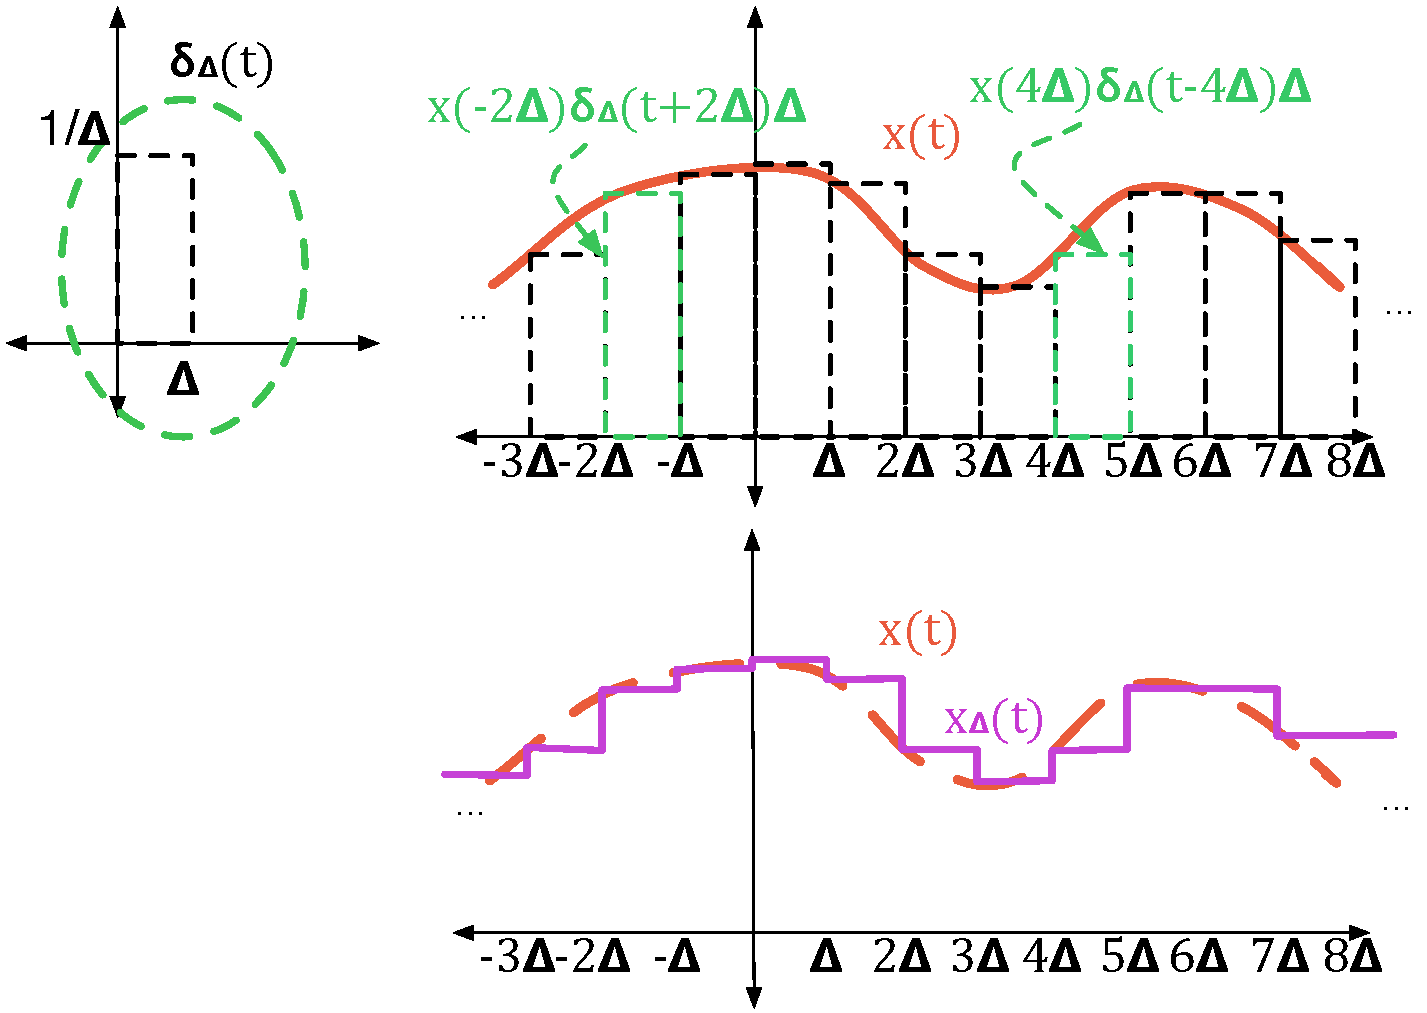
\includegraphics[scale=0.4]{Figures/Signal32.pdf}
\end{figure}
}

\frame{
\[
x(t) \approx x_{\Delta}(t) = \sum_{k=-\infty}^{\infty}{x(k\Delta){\color{blue}\delta_{\Delta}(t-k\Delta)}\Delta} 
\]
If we are able to compute the system's output for any  $\delta_{\Delta}(t-k\Delta)$
\begin{center}
\begin{pspicture}[](5,2)
   \pssignal(0,1){x}{$\delta_{\Delta}(t-k\Delta)$}
   \psblock(2,1){a}{L}
   %\psblock(4,1){b}{$h[n], H(z)$}
   \pssignal(4,1){y}{$h_{k\Delta}(t)$}
   %-----------------
   \psset{arrows=->}
   \ncline{x}{a}  \ncline{a}{y}  %\ncline{b}{y}
\end{pspicture}
\end{center}
\begin{figure}
\centering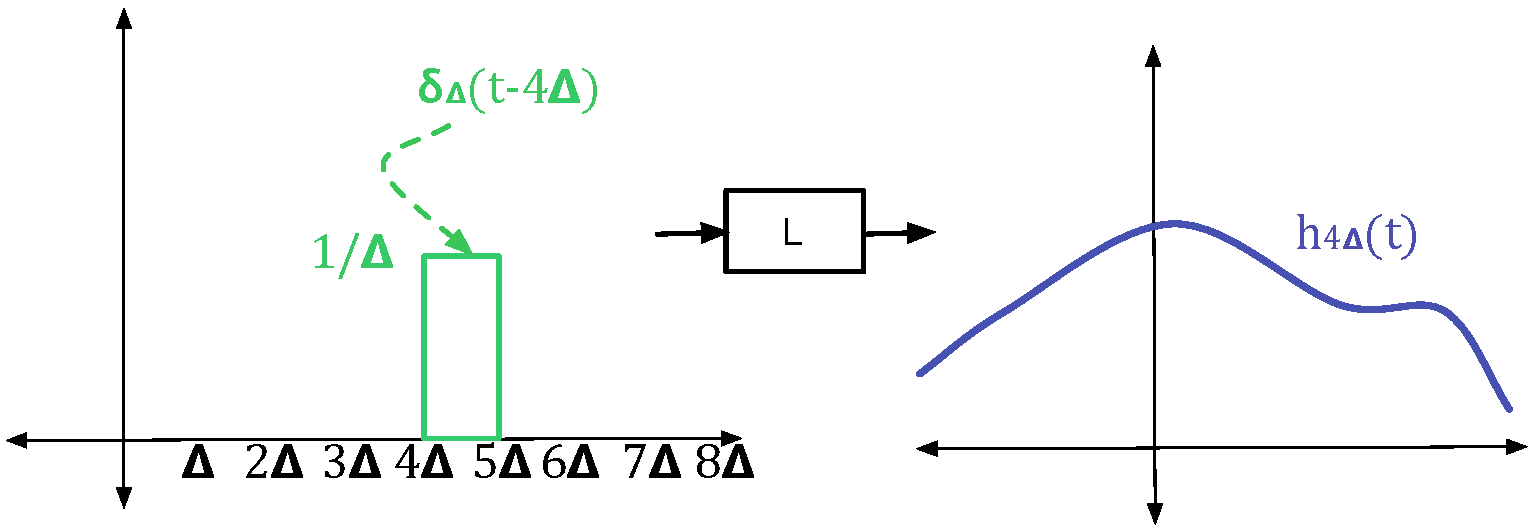
\includegraphics[scale=0.3]{Figures/Signal33.pdf}
\end{figure}

Then applying the superposition property
\begin{center}
\begin{pspicture}[](7,2)
   \pssignal(0,1){x}{$\displaystyle x_{\Delta}(t)$}
   \psblock(1.5,1){a}{L}
   %\psblock(4,1){b}{$h[n], H(z)$}
   \pssignal(6,1){y}{$y_{\Delta}(t) = \sum_{k=-\infty}^{\infty}{x(k\Delta) {\color{blue}h_{k\Delta}(t)}\Delta}$}
   %-----------------
   \psset{arrows=->}
   \ncline{x}{a}  \ncline{a}{y}  %\ncline{b}{y}
\end{pspicture}
\end{center}
}

\frame{
%El resultado anterior todavía es inmanejable porque depende de conocer infinitas $h_{k\Delta}(t)$
%
%\vspace{0.5cm}

If the system is also {\bf time-invariant}:
\begin{center}
\begin{pspicture}[](7,2)
   \pssignal(0,2){x}{$\delta_{\Delta}(t-k\Delta)$}
   \psblock(2,2){a}{LTI}
   %\psblock(4,1){b}{$h[n], H(z)$}
   \pssignal(5,2){y}{$h_{k\Delta}(t) = h_0(t-k\Delta)$}
   %-----------------
   \pssignal(0,1){x1}{$\displaystyle x_{\Delta}(t)$}
   \psblock(1.5,1){a1}{LTI}
   %\psblock(4,1){b}{$h[n], H(z)$}
   \pssignal(6,1){y1}{$y_{\Delta}(t) = \sum_{k=-\infty}^{\infty}{x(k\Delta) {\color{blue}h_0(t-k\Delta)}\Delta}$}
   \psset{arrows=->}
   \ncline{x}{a}  \ncline{a}{y}  %\ncline{b}{y}
     \ncline{x1}{a1}  \ncline{a1}{y1}	
\end{pspicture}
\end{center}

\vspace{0.5cm}

Taking the limit $\Delta \rightarrow 0$:
\begin{itemize}
\item $k\Delta \rightarrow \tau$
\item $\sum \rightarrow \int$
\item $\Delta \rightarrow d\tau$
\item $h_0(t) = h(t)$
\end{itemize}

\begin{exampleblock}{}
\begin{align}\nn
y(t) = \lim_{\Delta \rightarrow 0} y_{\Delta}(t) = \int_{-\infty}^{\infty}{x(\tau)h(t-\tau)d\tau}
\end{align}
\end{exampleblock}


}


%%%%%%%%%%%%%%%%%%%%%%%%%%%%%%%%%%%%%%%
% FIN EPH 20140222
%%%%%%%%%%%%%%%%%%%%%%%%%%%%%%%%%%%%%%%

%
%
%\frame{
%
%If the system's output is known for $\delta(t-\tau)$ for any $\tau\in\mathbb{R}$:
%
%\begin{center}
%\begin{pspicture}[](5,2)
%   \pssignal(0,1){x}{$\delta(t-\tau)$}
%   \psblock(2,1){a}{LTI}
%   %\psblock(4,1){b}{$h[n], H(z)$}
%   \pssignal(4,1){y}{$h_{\tau}(t)$}
%   %-----------------
%   \psset{arrows=->}
%   \ncline{x}{a}  \ncline{a}{y}  %\ncline{b}{y}
%\end{pspicture}
%\end{center}
%
%Then, by the superposition property,
%
%\begin{center}
%\begin{pspicture}[](7,2)
%   \pssignal(0,1){x}{$\displaystyle x(t)=\int_{-\infty}^{\infty}x(\tau)\delta(t-\tau)d\tau$}
%   \psblock(4,1){a}{LTI}
%   %\psblock(4,1){b}{$h[n], H(z)$}
%   \pssignal(6,1){y}{$y(t)$}
%   %-----------------
%   \psset{arrows=->}
%   \ncline{x}{a}  \ncline{a}{y}  %\ncline{b}{y}
%\end{pspicture}
%\end{center}
%
%\begin{exampleblock}{}
%\begin{align}\nn
%y(t)=\int_{-\infty}^{\infty} x(\tau)h_{\tau}(t) d\tau 
%\end{align}
%\end{exampleblock}
%
%}
%
%\frame{
%
%If the system is time-invariant:
%
%\begin{center}
%\begin{pspicture}[](7,2)
%   \pssignal(0,2){x}{$\delta(t)$}
%   \psblock(2,2){a}{LTI}
%   %\psblock(4,1){b}{$h[n], H(z)$}
%   \pssignal(5,2){y}{$h_{0}(t)=h(t)$}
%   
%    \pssignal(0,1){x1}{$\delta(t-\tau)$}
%   \psblock(2,1){a1}{LTI}
%   %\psblock(4,1){b}{$h[n], H(z)$}
%   \pssignal(5,1){y1}{$h_{\tau}(t)=h(t-\tau)$}  
%   %-----------------
%   \psset{arrows=->}
%   \ncline{x}{a}  \ncline{a}{y}  %\ncline{b}{y}
%   \ncline{x1}{a1}  \ncline{a1}{y1}
%\end{pspicture}
%\end{center}
%
%then, we finally obtain
%
%\begin{center}
%\begin{pspicture}[](7,2)
%   \pssignal(0,1){x}{$\displaystyle x(t)=\int_{-\infty}^{\infty}x(\tau)\delta(t-\tau)d\tau$}
%   \psblock(4,1){a}{LTI}
%   %\psblock(4,1){b}{$h[n], H(z)$}
%   \pssignal(6,1){y}{$y(t)$}
%   %-----------------
%   \psset{arrows=->}
%   \ncline{x}{a}  \ncline{a}{y}  %\ncline{b}{y}
%\end{pspicture}
%\end{center}
%
%\begin{exampleblock}{}
%\begin{align}\nn
%y(t)=\int_{-\infty}^{\infty} x(\tau)h(t-\tau) d\tau 
%\end{align}
%\end{exampleblock}
%
%}

\frame{

\begin{itemize}
\item $h(t)$ is the \textbf{system's response to the impulse $\delta(t)$}.
\item Any LTI system is \textbf{completely defined} by $h(t)$!
\vspace{0.3cm}
\begin{center}
\begin{pspicture}[](5,2)
   \pssignal(0,1){x}{$x(t)$}
   \psblock(2,1){a}{$h(t)$}
   %\psblock(4,1){b}{$h[n], H(z)$}
   \pssignal(4,1){y}{$y(t)$}
   %-----------------
   \psset{arrows=->}
   \ncline{x}{a}  \ncline{a}{y}  %\ncline{b}{y}
\end{pspicture}
\end{center}
\end{itemize}


\begin{block}{Continuous-time Convolution}
Given two signals $x(t)$ and $h(t)$:
\begin{align}\nn
\int_{-\infty}^{\infty} x(\tau)h(t-\tau) d\tau=x(t)\ast h(t)
\end{align}
is the continuous-time convolution operation between them.
\end{block}
}


\frame{
\frametitle{Problem 43}

Consider the two signals $x(t)$ and $h(t)$ given by:

\begin{align*}
x(t)=\left\{
\begin{array}{cc}
1 & 0< t< T\\
0 & \text{otherwise}
\end{array}
\right.,
\end{align*}

\begin{align*}
h(t)=\left\{
\begin{array}{cc}
t & 0< t< 2T\\
0 & \text{otherwise}
\end{array}
\right..
\end{align*}
If $h(t)$ is the impulse response of an LTI system,  compute the system's output when $x(t)$ is the input signal.


}

\frame{
\frametitle{Sol.}

\begin{center}
\begin{pspicture}[](5,2)
   \pssignal(0,1){x}{$x(t)$}
   \psblock(2,1){a}{$h(t)$}
   %\psblock(4,1){b}{$h[n], H(z)$}
   \pssignal(4,1){y}{$y(t)$}
   %-----------------
   \psset{arrows=->}
   \ncline{x}{a}  \ncline{a}{y}  %\ncline{b}{y}
\end{pspicture}
\end{center}

\begin{align*}
y(t)=\left\{
\begin{array}{cc}
0 & t<0\\
\frac{t^2}{2} & 0\leq t< T\\
tT-\frac{T^2}{2} & T\leq t <2T\\ 
Tt+\frac{3}{2}T^2-\frac{t^2}{2} &2T\leq t< 3T\\
0 & t\geq3T
\end{array}
\right.,
\end{align*}


}


\section{Properties of the Convolution operation}

%\frame{
%
%\begin{block}{Discrete-time Convolution}
%Given two discrete-time signals $x[n]$ and $h[n]$:
%\begin{align}\nn
%\sum_{k=-\infty}^{\infty}x[k]h[n-k]=x[n]\ast h[n]
%\end{align}
%is the convolution operation between them.
%\end{block}
%
%\begin{block}{Continuous-time Convolution}
%Given two signals $x(t)$ and $h(t)$:
%\begin{align}\nn
%\int_{-\infty}^{\infty} x(\tau)h(t-\tau) d\tau=x(t)\ast h(t)
%\end{align}
%is the continuous-time convolution operation between them.
%\end{block}
%
%}

\frame{
\frametitle{Commutative property}

\begin{exampleblock}{}
\begin{align}\nn
x[n]\ast h[n]=h[n]\ast x[n]
%\Rightarrow \sum_{k=-\infty}^{\infty}x[k]h[n-k]=\sum_{k=-\infty}^{\infty}h[k]x[n-k]
\end{align}
\end{exampleblock}

\textbf{Proof.:}

Given 
\begin{align}\nn
x[n]\ast h[n]=\sum_{k=-\infty}^{\infty}x[k]h[n-k]
\end{align}
define $v=n-k$, thus
\begin{align}\nn
x[n]\ast h[n]=\sum_{v=+\infty}^{-\infty}x[n-v]h[v]=\sum_{v=-\infty}^{+\infty}h[v]x[n-v]=h[n]\ast x[n]
\end{align}
}



\frame{
\frametitle{Commutative property}
Therefore,
\begin{center}
\begin{pspicture}[](5,2)
   \pssignal(0,1){x}{$x[n]$}
   \psblock(2,1){a}{$h[n]$}
   %\psblock(4,1){b}{$h[n], H(z)$}
   \pssignal(4,1){y}{$y[n]$}
   %-----------------
   \psset{arrows=->}
   \ncline{x}{a}  \ncline{a}{y}  %\ncline{b}{y}
\end{pspicture}
\end{center}
is equivalent to
\begin{center}
\begin{pspicture}[](5,2)
   \pssignal(0,1){x}{$h[n]$}
   \psblock(2,1){a}{$x[n]$}
   %\psblock(4,1){b}{$h[n], H(z)$}
   \pssignal(4,1){y}{$y[n]$}
   %-----------------
   \psset{arrows=->}
   \ncline{x}{a}  \ncline{a}{y}  %\ncline{b}{y}
\end{pspicture}
\end{center}

\begin{exampleblock}{Commutative property for the continuous-time convolution}
\begin{align}\nn
x(t)\ast h(t)=h(t)\ast x(t)\Rightarrow \int_{-\infty}^{\infty} x(\tau)h(t-\tau) d\tau=\int_{-\infty}^{\infty} h(\tau)x(t-\tau) d\tau
\end{align}
\end{exampleblock}

}

\frame{
\frametitle{Associative property}

\begin{align}\nn
x(t)\ast \Big(h(t) \ast z(t)\Big)=\Big(x(t)\ast h(t)\Big)  \ast z(t)\\\nn\\\nn
x[n]\ast \Big(h[n] \ast z[n]\Big)=\Big(x[n]\ast h[n]\Big)  \ast z[n]
\end{align}
Therefore, the following configurations are equivalent:

\begin{center}
\begin{pspicture}[](8,2)
   \pssignal(0,1){x}{$x(t)$}
   \psblock(2,1){a}{$h_1(t)$}
   \psblock(5,1){b}{$h_2(t)$}
   \pssignal(8,1){y}{$y(t)$}
   %-----------------
   \psset{arrows=->}
   \ncline{x}{a}  \ncline{a}{b}  \ncline{b}{y}
\end{pspicture}
\vspace{0.5cm}

\begin{pspicture}[](7,2)
   \pssignal(0,1){x}{$x(t)$}
   \psblock(3,1){a}{$h_1(t)\ast h_2(t)$}
   %\psblock(4,1){b}{$h[n], H(z)$}
   \pssignal(6,1){y}{$y(t)$}
   %-----------------
   \psset{arrows=->}
   \ncline{x}{a}  \ncline{a}{y}  %\ncline{b}{y}
\end{pspicture}
\vspace{0.5cm}

\begin{pspicture}[](8,2)
   \pssignal(0,1){x}{$x(t)$}
   \psblock(2,1){a}{$h_2(t)$}
   \psblock(5,1){b}{$h_1(t)$}
   \pssignal(8,1){y}{$y(t)$}
   %-----------------
   \psset{arrows=->}
   \ncline{x}{a}  \ncline{a}{b}  \ncline{b}{y}
\end{pspicture}
\end{center}

}

\frame{
\frametitle{Distributive property with respect to the sum}
\begin{align}\nn
x[n]\ast\Big(y[n]+z[n]\Big)=x[n]\ast y[n]+x[n]\ast z[n]\\\nn\\\nn
x(t)\ast\Big(y(t)+z(t)\Big)=x(t)\ast y(t)+x(t)\ast z(t)
\end{align}
The following configurations are equivalent:

\begin{center}
\begin{pspicture}[](6.5,2)	
   \pssignal(0,1){x}{$x(t)$}
   \pnode(1,1){b}
   \pnode(1,2){c}
   \pnode(1,0){d}
   \psblock(3,2){e}{$h_1(t)$}
   \psblock(3,0){f}{$h_2(t)$}
   \pnode(5,2){g}
   \pnode(5,0){h}
   \pscircleop(5,1){oplus}
   \pssignal(6.25,1){i}{$y(t)$}
   \ncline{x}{b}  \ncline{b}{c}  \ncline{b}{d}
    \ncline{e}{g} \ncline{f}{h}
   \psset{style=RoundCorners ,style=Arrow}
     \ncline{c}{e} \ncline{d}{f}
   \ncline{g}{oplus}  \ncline{h}{oplus} \ncline{oplus}{i}
\end{pspicture}
\vspace{1cm}

\begin{pspicture}[](5,2)
   \pssignal(-1,1){x}{$x(t)$}
   \psblock(2,1){a}{$h_1(t)+ h_2(t)$}
   %\psblock(4,1){b}{$h[n], H(z)$}
   \pssignal(5,1){y}{$y(t)$}
   %-----------------
   \psset{arrows=->}
   \ncline{x}{a}  \ncline{a}{y}  %\ncline{b}{y}
\end{pspicture}
\end{center}
}

\frame{
\frametitle{Convolution with an impulse signal}

Remember that any signal can be decomposed as a linear combination of an infinite number of unit impulses:

\begin{align}\nn
x[n]&=\sum_{k=-\infty}^{\infty}x[k]\delta[n-k],\\\nn
x(t)&=\int_{-\infty}^{\infty}x(\tau)\delta(t-\tau)d\tau
\end{align}

Therefore
\begin{alertblock}{}
\begin{align}
x[n]\ast \delta[n]=x[n],\nn\\\nn
x(t)\ast \delta(t)=x(t).
\end{align}
\end{alertblock}

}


\frame{
\frametitle{Convolution with a delayed  impulse (discrete-time)}

\begin{align}\nn
x[n]\ast \delta[n-n_0]=\sum_{k=-\infty}^{\infty}x[k]\delta[n-k-n_0]
\end{align}
Define $v=k+n_0$, thus
\begin{align}\nn
x[n]\ast \delta[n-n_0]&=\sum_{v=-\infty}^{\infty}x[v-n_0]\delta[n-v]\\\nn
&=x[n-n_0]\ast \delta[n]=x[n-n_0].
\end{align}

Therefore,
\begin{block}{}
\begin{align}
x[n]\ast \delta[n-n_0]=x[n-n_0],\nn\\\nn
%x(t)\ast \delta(t-t_0)=x(t-t_0).
\end{align}
\end{block}


}

\frame{
\frametitle{Convolution with a delayed  impulse (continuous-time)}

\begin{align}\nn
x(t)\ast \delta(t-t_0)=\int_{\tau=-\infty}^{\infty}x(\tau)\delta(t-\tau-t_0)\text{d}\tau
\end{align}
Define $v=\tau+t_0$ and $x'(t)=x(t-t_0)$, thus
\begin{align*}
x(t)\ast \delta(t-t_0)&=\int_{v=-\infty}^{\infty}x(v-t_0)\delta(t-v)\text{d}v\\
&=\int_{v=-\infty}^{\infty}x'(v)\delta(t-v)\text{d}v=x'(t)\ast \delta(t)=x'(t)
\end{align*}

Therefore,
\begin{block}{}
\begin{align}
x(t)\ast \delta(t-t_0)=x(t-t_0),\nn\\\nn
%x(t)\ast \delta(t-t_0)=x(t-t_0).
\end{align}
\end{block}


}



\end{document}
